\documentclass[12pt,a4paper]{article}
\usepackage[margin=2.5cm,bottom=3cm,foot=1.5cm]{geometry}
\setlength{\parindent}{0pt}
\setlength{\parskip}{0.6ex}

\usepackage{graphicx}
\usepackage{subfig}
\usepackage{caption}
\usepackage{multirow}
\usepackage{multicol}
\usepackage{amsmath}
\usepackage{amssymb}
\usepackage{amsfonts}
\usepackage{mathrsfs}
\usepackage[usenames]{color}
\usepackage[english]{babel}
\usepackage[utf8]{inputenc}
\usepackage{siunitx}
\usepackage{float}
\usepackage{physics}

\usepackage[style=nature, backend=biber, sorting=none]{biblatex}
\bibliography{qa.bib}

\def\phi{\varphi}
\def\eps{\varepsilon}
\def\theta{\vartheta}

\renewcommand{\Re}{\mathop{\rm Re}\nolimits}
\renewcommand{\Im}{\mathop{\rm Im}\nolimits}
\newcommand{\diag}{\mathop{\rm diag}\nolimits}
\newcommand{\ddd}{\mathrm{d}}
\newcommand{\ii}{\mathrm{i}}
\newcommand{\lag}{\mathcal{L}\!}
\newcommand{\ham}{\mathcal{H}\!}
\newcommand{\four}[1]{\mathcal{F}\!\left(#1\right)}
\newcommand{\bigO}[1]{\mathcal{O}\!\left(#1\right)}
\newcommand{\sh}{\mathop{\rm sinh}\nolimits}
\newcommand{\ch}{\mathop{\rm cosh}\nolimits}
\renewcommand{\th}{\mathop{\rm tanh}\nolimits}
\newcommand{\erfc}{\mathop{\rm erfc}\nolimits}
\newcommand{\sinc}{\mathop{\rm sinc}\nolimits}
\newcommand{\rect}{\mathop{\rm rect}\nolimits}
\newcommand{\ee}[1]{\cdot 10^{#1}}
\newcommand{\inv}[1]{\left(#1\right)^{-1}}
\newcommand{\invf}[1]{\frac{1}{#1}}
\newcommand{\sqr}[1]{\left(#1\right)^2}
\newcommand{\half}{\frac{1}{2}}
\newcommand{\thalf}{\tfrac{1}{2}}
\newcommand{\pd}{\partial}
\newcommand{\plag}[1]{\frac{\partial \mathcal{L}}{\partial #1}}
\newcommand{\Dd}[3][{}]{\frac{\ddd^{#1} #2}{\ddd #3^{#1}}}
\newcommand{\Pd}[3][{}]{\frac{\pd^{#1} #2}{\pd #3^{#1}}}
\newcommand{\avg}[1]{\left\langle#1\right\rangle}
\newcommand{\obraket}[3]{\left\langle #1 \vert #2 \vert #3 \right \rangle}
\newcommand{\hex}[1]{\texttt{0x#1}}

\newcommand{\oiint}{\mathop{{\int\mkern-15mu\int}\mkern-21mu\raisebox{0.3ex}{$\bigcirc$}}}

\newcommand{\wunderbrace}[2]{\vphantom{#1}\smash{\underbrace{#1}_{#2}}}

\renewcommand{\vec}[1]{\overset{\smash{\hbox{\raise -0.42ex\hbox{$\scriptscriptstyle\rightharpoonup$}}}}{#1}}
\newcommand{\bec}[1]{\mathbf{#1}}


\begin{document}


\begin{titlepage}
    \begin{center}
        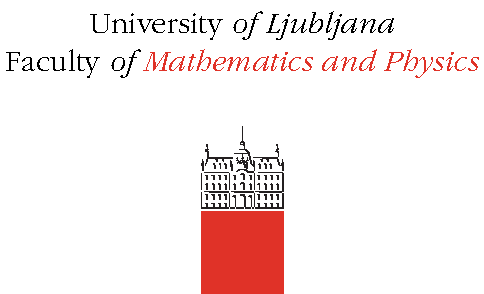
\includegraphics[width=0.4\textwidth]{../plots/logo_fmf_uni-lj_en.pdf}
            
        \vspace{1cm}    
        
        \large{Masters program in Physics}\\
        \large{Seminar 2}\\
        \vspace{2cm}
        \Large\textbf{Using quantum annealing for equilibrium quantum simulation}
            
        \vspace{1.5cm}
            
        \large{Author: Vid Eržen} \\
        \large{Advisor: Prof. Dr. Dragan Mihailović} \\
        \large{Co-advisor: Dr. Jaka Vodeb}

        \vspace{0.5cm}
            
        Ljubljana, February 2024
            
        \vspace{1.5cm}   
        
        \subsection*{Abstract}

    \end{center}
    \hspace*{0.3cm}
    We present quantum annealing, an algorithm that was initially developed
    for solving combinatorial optimization problems, but is becoming increasingly important as a
    quantum simulator. We begin with a brief overview of optimization problems and discuss how the adiabatic
    theorem of quantum mechanics can be used to solve them. Once the construction of the quantum annealing Hamiltonian
    is justified, we shift our focus from optimization problems to equilibrium simulations of quantum systems.
    We describe how the interaction between quantum annealers and their environment enables sampling states from
    the Boltzmann/thermal distribution, associated with the annealing Hamiltonian and the temperature of the
    environment. We then discuss the protocol for producing such samples with quantum annealers and conclude the
    seminar with a review of quantum Monte Carlo methods, classical algorithms for simulating quantum annealers. 
\end{titlepage}
\vspace{-1cm}


\tableofcontents

\section{Introduction} \label{sec:intro}
\hspace*{0.3cm}
Understanding magnetic phases in quantum mechanical systems is one of the main goals in condensed matter physics,
and the advent of quantum simulation hardware has provided new tools for experimentally probing such systems~\cite*{harris2018phase}.
General purpose or gate model quantum computers are are hard to scale up, with the
current devices being limited to a few hundreds of qubits and are therefore not yet able to simulate
large quantum systems. Even worse, for a reliable simulation,
one would need to use error correction codes, which is a huge overhead, because many physical qubits are
needed to encode a single logical qubit, which is then used to represent a degree of freedom, like a spin on a lattice~\cite*{preskill2018quantum}.
Given these challenges, researchers have searched for less demanding, but possibly specialized alternatives,
which may be able to solve certain problems of practical importance.
One such alternative, initially developed for solving combinatorial optimization problems, is quantum annealing~\cite*{hauke2020perspectives}. This algorithm is becoming increasingly important as a quantum simulator, and here we review the algorithm and show how it can be used for equilibrium simulations of quantum systems,
e.g. calculating the phase diagram of a transverse field Ising model (TFIM) on a cubic lattice. 
Before discussing how such simulations can be performed on a quantum annealer,
we first differentiate between quantum annealing and the universal (gate) model of quantum computing.


\subsection*{Quantum annealing and gate model} \label{sec:qa_vs_gate}

\hspace*{0.3cm}
The gate model of quantum computing is a universal model of quantum computation. If we view computation
as a process of transforming an input to an output, then the gate model is universal in a sense that it can
approximate any such transformation to arbitrary precision. The name comes from the fact
it does this by applying a sequence of quantum gates on a single qubit or a pair of qubits.
We can therefore classify it as a digital computational model.

\hspace*{0.3cm}
Quantum annealing (QA) on the other hand, is an analog quantum algorithm. Rather than applying a sequence of
quantum gates on a state, it evolves an input state according to a time-dependent Hamiltonian, with different choices
of Hamiltonian mapping the input state to different output states. For this reason, the Hamiltonian
is usually parametrized by a few programmable parameters, which allows us to perform different computations~\cite*{albash2018adiabatic}.
A candidate system for QA might be spins on a lattice, whose time evolution is governed by the Heisenberg
Hamiltonian with programmable interaction strengths and local magnetic fields.

\hspace*{0.3cm}
Even though quantum annealers can only represent a certain class of Hamiltonians,
it was shown that this algorithm is equivalent to the universal gate model of quantum computing~\cite{aharonov2008adiabatic},
provided the Hamiltonian is general enough (e.g. the Heisenberg Hamiltonian). This means that any problem that can
be solved on a gate model computer can also be solved on a quantum annealer with at most a polynomial overhead.
Because of this, we can say that quantum annealing is not an algorithm, but a computational model.

\hspace*{0.3cm}
In practice, however, most quantum annealers only use a certain class of Hamiltonians, called \textit{stoquastic} Hamiltonians,
which renders quantum annealing less powerful than the gate model~\cite*{crosson2021prospects}.
The most widely used stoquastic Hamiltonian in quantum annealers is the transverse field Ising model (TFIM),
which is the focus of Section \ref{sec:qa}. We see the first limitation of quantum annealers --- they are only
able to represent a certain class of Hamiltonians, which restricts
the number of simulable systems. This might seem extremely restrictive, but quantum annealers have been
successfully used to observe a number of interesting phenomena. Focusing only on the equilibrium simulations
of physical systems, some well-known examples are the phase diagram
of the TFIM on a cubic lattice~\cite*{harris2018phase}, the Kosterlitz-Thouless
phase transition of the TFIM on a geomatrically frustrated lattice~\cite*{king2018observation}, and more exotic
phase diagrams, like the Shastry-Sutherland model~\cite*{kairys2020simulating}.
Especially interesting are problems that are not exclusively tied to the TFIM, like the Kosterlitz-Thouless
transition, where TFIM serves only as a testbed for the implementation of a more general phenomenon.

\hspace*{0.3cm}
Due to the stoquasticity of TFIM, equilibrium properties of quantum annealers can be usually efficiently
simulated on a classical computer using quantum Monte Carlo (QMC) methods~\cite*{bravyi2006complexity}.
This is one of the reasons for the shift of focus of research on quantum annealers towards
simulating the dynamics of quantum systems, in hope to perform a computation that is infeasible for classical
computers - to demonstrate quantum supremacy~\cite*{king2024computational}.

\hspace*{0.3cm}
The paper is organized as follows. In Section \ref{sec:ising}, we briefly discuss optimization problems,
as they provide a natural motivation for introducing the quantum annealing algorithm and explain why the
transverse field Ising model Hamiltonian is the most widely used Hamiltonian for quantum annealers.
Section \ref{sec:qa} follows up with a review of the adiabatic theorem of quantum mechanics and discusses how it
can be used to solve optimization problems. Once the construction of the quantum annealing Hamiltonian is justified,
we shift our focus from optimization problems to equilibrium simulations of quantum systems in
Section \ref{sec:equilibrium_simulations}. We begin by stressing the importance of sampling
from the thermal distribution for such simulations and discuss how the interaction between quantum annealers
and their environment enables it, and then we explain the protocol
for thermal sampling on quantum annealers. We conclude with a discussion about
how the stoquasticity of the annealing Hamiltonian enables an efficient simulation of quantum annealers
on classical computers.

\section{Universality of Ising model} \label{sec:ising}
\hspace*{0.3cm}
Historically, the main motivation for introducing quantum annealing was to solve combinatorial optimization problems~\cite*{farhi2000quantum}.
A simple and instructive example of an optimization problem is the graph partitioning problem. Given a graph $G = (V, E)$, where $V$ is the set of vertices
and $E$ is the set of edges, the goal is to partition the vertices into two sets $A$ and $B$ such that the number of edges
between the two sets is minimized (Fig. \ref{fig:graph_partitioning}).
\begin{figure}[!htb]
    \centering
    \vspace*{-0.2cm}
    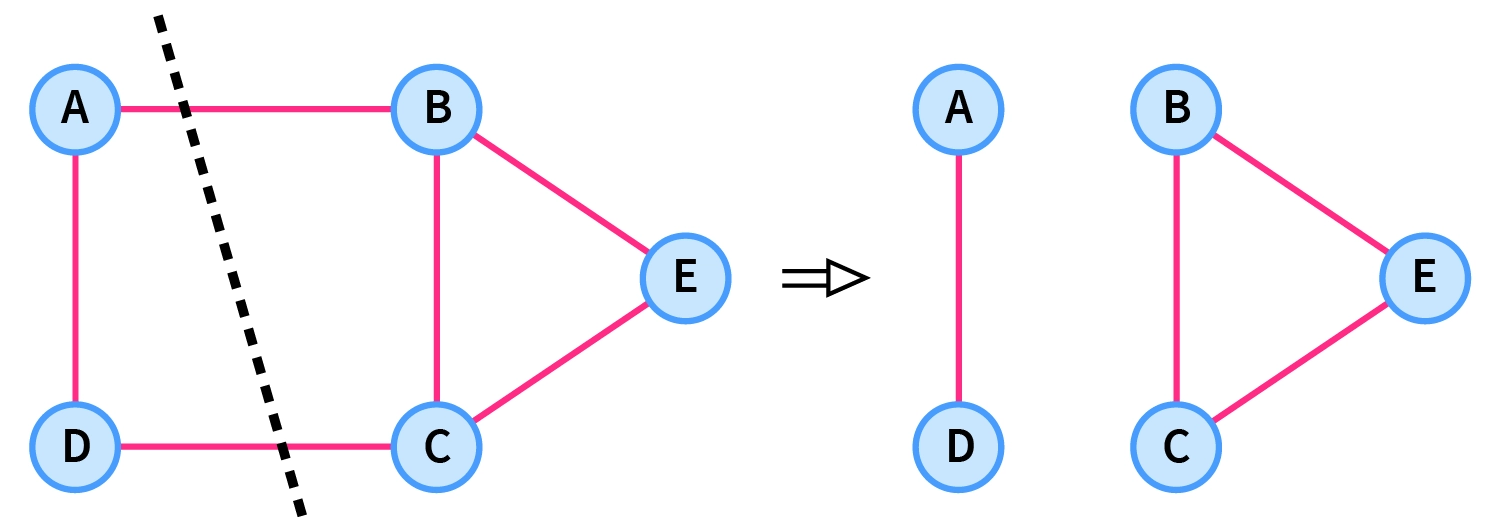
\includegraphics[width=0.5\textwidth]{../plots/min_cut.png}
    \captionsetup{width=0.9\textwidth}
    \caption{An example of the graph partitioning problem. The objective is to cut the graph into two sets,
    such that the number of links/edges between the two sets is minimized.}
    \label{fig:graph_partitioning}
\end{figure}
This problem can arise in many situations, like dividing a social network or
splitting a sparse matrix into parts, which can then be used to parallelize matrix operations. 

\hspace*{0.3cm}
The graph partitioning problem can be solved by introducing a spin variable $s_i = \pm 1$ at each vertex, with $s_i = 1$ if $i \in A$ and
$s_i = -1$ if $i \in B$, and finding a configuration of spins $\{s_i\}$
that minimizes the number of edges between the two sets
\begin{equation}
    H =  \sum_{(ij) \in V} \frac{1 - s_i s_j}{2}.
    \label{eq:graph_partitioning}
\end{equation}
Each edge contributes 1 to the energy if the spins at its ends are different and 0 if they are the same. Function
$H$ therefore counts the number of edges between the two partitions, which we would like to minimize.

\hspace*{0.3cm}
In general, many optimization problems of practical importance, like job scheduling problems~\cite{venturelli2015quantum},
the travelling saleseman problem~\cite{martovnak2004quantum}, search engine ranking~\cite{garnerone2012adiabatic}
or protein folding~\cite{perdomo2012finding}, can be phrased as finding the ground state of a
classical Ising Hamiltonian
\begin{equation}
    H_P = \sum_i h_i s_i + \sum_{i,j} J_{ij} s_i s_j,
    \label{eq:ising_ham}
\end{equation}
where the subscript $P$ stands for problem whereas $J_{ij}$ and $h_i$ are arbitrary parameters that specify the optimization
problem, which we call couplings and bias magnetic fields, respectively. In this sense, finding the ground state
of a classical Ising Hamiltonian is a universal combinatorial optimization problem~\cite*{lucas2014ising}.
In the next section, we describe how quantum annealing can be used to solve it.



\section{Quantum annealing} \label{sec:qa}

\hspace*{0.3cm}
Quantum annealing exploits the adiabatic theorem of quantum mechanics
to find the ground state of the problem Hamiltonian [Eq. \eqref{eq:ising_ham}] and we begin
by reviewing the theorem. 

\subsection*{The adiabatic theorem} \label{sec:adiabatic}
\hspace*{0.3cm}
The theorem roughly states that if a quantum system is prepared in the ground state of a Hamiltonian $H_0$
and the Hamiltonian is changed sufficiently slowly to a new Hamiltonian $H_P$, the system will remain in the
ground state of the new Hamiltonian~\cite*{albash2018adiabatic}. We can immediately see how this can be used to find the ground state
if the Ising Hamiltonian [Eq. \eqref{eq:ising_ham}]: If we start with a Hamiltonian $H_0$ whose ground state is
easy to prepare experimentaly and then slowly change it to the Ising Hamiltonian $H_P$ whose ground state encodes the
solution to an optimization problem, the system will end up the ground state of $H_P$ and
we will have found the solution to the optimization problem. Let us now formalize this idea.

\hspace*{0.3cm}
Denote the full annealing time as $T$, introduce a dimensionless time
parameter $s = t / T$, and write a general time-dependent annealing Hamiltonian as
\begin{equation}
    H(s) = A(s) H_0 + B(s) H_P,
    \label{eq:QA_ham}
\end{equation}
where $A(s)$ and $B(s)$ are time-dependent functions that satisfy $A(0) = 1$, $B(0) = 0$, $A(1) = 0$, and $B(1) = 1$.
We must also require that $H_0$ and $H_P$ do not commute in order to exploit quantum mechanical tunneling effect. If they did
commute, we could diagonalize both $H_0$ and $H_P$ at once, which would make the whole Hamiltonian diagonal
in some basis --- there would be no off-diagonal elements and therefore no transitions and tunneling between states.
Because we are introducing quantum mechanics into a classical Ising system,
we should also promote the classical spins to quantum spin-1/2 systems. Somewhat schematically, we can denote
this with renaming $s_i \to \sigma^z_i$ in the Ising Hamiltonian [Eq. \eqref{eq:ising_ham}], where $\sigma^z_i$ is a
Pauli matrix acting on the $i$-th spin.

\hspace*{0.3cm}
The adiabatic theorem states that if the annealing time $T$ is large enough compared to the
energy gap $\Delta$ between the ground state and the first excited state,
the system will remain in the ground state of $H_P$ at the end of the annealing process
with high probability. Specifically, if (setting $\hbar = 1$)
\begin{equation}
    T \gg \max_{0 \leq s \leq 1} \frac{\left| \mel{1(s)}{\frac{\pd H}{\pd s}}{0(s)} \right|}{\Delta(s)^2},
    \label{eq:adiabatic_theorem}
\end{equation}
the probability of the system being in the ground state of $H_P$ at the end of the annealing process
is close to unity~\cite{albash2018adiabatic}. Here $\ket{0(s)}$ and $\ket{1(s)}$ are the instantaneous ground and the
first excited state of $H(s)$, respectively. All that is left to do is to choose the initial Hamiltonian $H_0$
and we will have constructed a quantum annealer.


\subsection*{Quantum annealing Hamiltonian} \label{sec:qa_ham}

\hspace*{0.3cm}
In order to use quantum annealing to solve optimization problems, we need to choose the initial Hamiltonian $H_0$.
This should be a Hamiltonian whose ground state is easy to prepare and it should not commute with
the problem Hamiltonian $H_P$. The simplest choice which satisfies these requirements, is the
transverse field Hamiltonian
\begin{equation}
    H_0 = - \sum_i \sigma^x_i,
    \label{eq:transverse_ham}
\end{equation}
where $\sigma^x_i$ is a Pauli matrix acting on the $i$-th spin. The ground state of $H_0$ is the uniform superposition
of all possible spin configurations, $\ket{+++\ldots}$, where $\ket*{+} = \frac{1}{\sqrt{2}}(\ket*{0} + \ket*{1})$.
In order to prepare this ground state, one should only apply a strong enough transverse magnetic field $A(s)$
to the system, which will align all spins in the $x$ direction. Another intuitive reason for choosing the transverse
field Hamiltonian [Eq. \eqref{eq:transverse_ham}] as the initial Hamiltonian is that the ground state, after applying
the Born rule, is a uniform probability distribution over all possible final configurations, which is the most
unbiased initial state that we can prepare.

\hspace*{0.3cm}
The full annealing Hamiltonian is then given by
\begin{equation}
    H(s) = - A(s) \sum_i \sigma^x_i + B(s) \left( \sum_i h_i \sigma^z_i + \sum_{i,j} J_{ij} \sigma^z_i \sigma^z_j \right).
    \label{eq:QA_ham_full}
\end{equation}
In Fig. \ref{fig:spectrum}, we see a typical spectrum of this Hamiltonian [Eq. \eqref{eq:QA_ham_full}]
for a simple one-dimensional Ising chain with 3 spins, randomly chosen $h_i$ and $J_{ij}$ and $A(s) = 1 - s$ and $B(s) = s$.
\begin{figure}[!htb]
    \centering
    \vspace*{-0.3cm}
    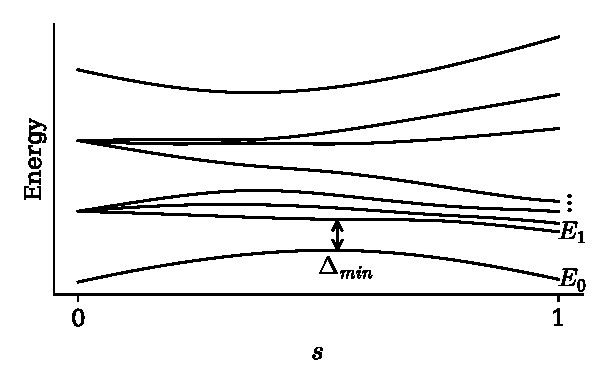
\includegraphics[width=0.55\textwidth]{../plots/ising_gap.pdf}
    \captionsetup{width=0.9\textwidth}
    \vspace*{-0.4cm}
    \caption{The energy spectrum of the annealing Hamiltonian [Eq. \eqref{eq:QA_ham_full}] for a
    one-dimensional transverse field Ising chain with 3 spins and randomly chosen $h_i$ and $J_{ij}$,
    $A(s) = 1 - s$ and $B(s) = s$.}
    \label{fig:spectrum}
\end{figure}

\hspace*{0.3cm}
The adiabatic theorem [Eq. \eqref{eq:adiabatic_theorem}] states that the system will remain in the ground state of the annealing Hamiltonian
if annealing is slow enough compared to the minimum energy gap $\Delta_{min}$.
Fig. \ref{fig:spectrum} motivates us to promote the dimensionless time parameter $s=t/T$ to an arbitrary function of time $s(t)$
[still obeying $s(0) = 0$ and $s(T) = 1$]. This enables us to choose annealing to be fast when the gap is
large and slow when the gap is small. In this way, we can increase the computational power of QA. We call
this function the annealing schedule; this is one of the most important parameters of the quantum annealer.
Famously, it was shown that a non-linear annealing schedule is required to obtain a quadratic speedup
over classical computers for the problem of searching for an element in an unsorted list~\cite{roland2002}.
This is equivalent to the quadratic speedup of Grover's algorithm for the same task on the gate model quantum computers.

\hspace*{0.3cm}
So far, we constructed the most widely used quantum annealing Hamiltonian in order to solve optimization problems.
We began by showing that most optimization problems can be phrased as finding the ground state of a classical Ising
Hamiltonian [Eq. \eqref{eq:ising_ham}], with couplings $J_{ij}$ and bias magnetic fields $h_i$ specifying the problem.
We then postulated the complete annealing Hamiltonian [Eq. \eqref{eq:QA_ham_full}] based on simplicity, non-commutativity
with the Ising Hamiltonian, and the fact that the ground state of the initial Hamiltonian is easy to prepare
experimentally. In the end, we showed that the annealing schedule $s(t)$ should be programmable as well
in order to achieve certain computational speedups over classical computers. Thus we constructed a quantum annealer
with 3 sets of programmable parameters: Local magnetic fields $h_i$, couplings $J_{ij}$, and the custom annealing schedule $s(t)$.

\hspace*{0.3cm}
We now change the focus from optimization problems and discuss how such devices can be used by physicists
to simulate equilibrium properties of quantum systems. In particular, we will be concerned with
the thermal sampling on quantum annealers and we will show how it can be used to calculate the expectation values of observables
at different physical parameters. This will in turn allow us to study magnetic phase diagram of the TFIM.


\section{Equilibrium physics simulations} \label{sec:equilibrium_simulations}
\hspace*{0.3cm}
When a system is in a thermal equilibrium with the environment at temperature $T$, we do not know its exact state,
but we know the probability distribution over its energy eigenstates $\{\psi_i\}$ with energies $\{E_i\}$.
It is given by the Boltzmann weights 
\begin{equation}
    p_i = \exp(- \beta E_i) / Z,
    \label{eq:boltzmann}
\end{equation}
where $Z = \sum_i \exp(-\beta E_i)$ is the partition function and $\beta = 1 / k_B T$
is the inverse temperature. Because we only know the probability distribution over possible states,
the observables, like magnetization or magnetic susceptibility, will also
be distributed according to some distribution. The simplest questions that we can ask about the system of interest
then concern the expectation values of those observables at different parameters.
We can calculate them analytically for a few simple models, but this is not possible in general.
In those cases, we have to resort to numerical methods, which allow us to draw samples from the thermal
distribution [Eq. \eqref{eq:boltzmann}] and estimate the expectation values of observables.
Let us denote the number of obtained samples by $N$, samples by $\{s_i\}$ and the observable by $O$.
The expectation value of the observable is then given by
\begin{equation}
    \avg{O} := \sum_i p_i \mel{\psi_i}{O}{\psi_i} \underset{N \to \infty}{\approx} \frac{1}{N} \sum_{n=1}^N O(s_n).
    \label{eq:expectation_value}
\end{equation}
The number of terms in the first sum of Eq.~\eqref{eq:expectation_value} grows exponentially with the
number of lattice sites and is therefore not practical to compute for large systems. The approximation
in the last step in Eq.~\eqref{eq:expectation_value} denotes the Monte Carlo method which has the advantage that the number of samples $N$ needed to bound
the variance of the estimated observable often grows polynomially with the number of lattice sites, and we can use it
to compute the expectation values of observables for large systems.

\hspace*{0.3cm}
For decades, the most widely used methods for producing samples from the thermal distribution were the
Metropolis-Hastings algorithm and its variants~\cite*{izquierdo2021testing}. With the advent of quantum annealers, we can
use them for sampling as well. So far, however, we have only discussed quantum annealers as closed systems,
which means that there are no fluctuations from the environment, the system is in a pure state and there is
no well defined notion of temperature. Therefore, isolated quantum annealers can not be used
to draw samples from the thermal distribution.


\subsection*{Physical implementation} \label{sec:physical_implementation}
\hspace*{0.3cm}
As stated, quantum annealers by themselves can not be used as thermal samplers. Luckily, physical devices
are never completely isolated from the environment, which introduces noise and effectively
adds a temperature to the system. If the coupling between the system and the environment is strong enough,
we can assume that the system is in a thermal state associated with the TFIM Hamiltonian [Eq. \eqref{eq:QA_ham_full}]
at the temperature of the environment $T$, and so we can measure the system and in this way obtain samples from the thermal distribution.
This is not a trivial assumption, but an open-system adiabatic theorem 
provides a guarantee that if we wait long enough, the state of the system will approach the desired
thermal state~\cite*{venuti2016adiabaticity}. The coupling to the environment
should not be too strong in order to approximately preserve the spectrum of the TFIM Hamiltonian.

\hspace*{0.3cm}
An example of the implementation of the quantum annealer that we will focus on
is based on superconducting qubits. This is the most widely used platform for quantum annealing
and we also have cloud access to some of the devices, made by the D-Wave company.

\hspace*{0.3cm}
In the current generation of D-Wave devices, there are more than 5000 qubits, each coupled to 15 other qubits
through flux-tunable couplers. This is, for example, enough to embedd a $15 \times 15 \times 12$ cubic
lattice onto the quantum processing unit (QPU). The QPU is a chip which lies in a dilution refrigerator
and is cooled to approximately \SI{15}{mK}, which sets the temperature scale of the system.
The temperature itself is not tunable, but we can effectively change
it by modifying the energy scale of the system --- changing coupling strengths $\{J_{ij}\}$ and magnetic fields $\{h_i\}$.
With this in mind, we can finally discuss thermal sampling on quantum annealers.


\subsection*{Sampling on quantum annealers} \label{sec:sampling_on_qa}
\hspace*{0.3cm}
The system we will focus on here, is the TFIM on the cubic lattice with $J_{ij} = J$ and $h_i = 0$.
In order to perform the experiment, we must first map the cubic lattice onto the graph,
formed by the qubits and couplers on the QPU. We then choose the simulation parameters, temperature $T$ and
the dimensionless strength of the transverse field $A(s) / B(s)$, and we determine the programmable parameters $J$ and $s$
to match the simulation parameters. The crucial part of the experiment is the customizable annealing schedule $s(t)$,
which, as we argued in Section \ref{sec:qa}, should be a feature of any quantum annealer in order to
achieve certain computational speedups over classical computers. In this section, we will leverage
this capability in order to produce thermal samples.

\hspace*{0.3cm}
The annealing schedule of choice for thermal sampling is called the pause annealing schedule
shown in Fig.~\ref{fig:pause_anneal_schedule}.
\begin{figure}[!htb]
    \vspace*{-0.2cm}
    \centering
    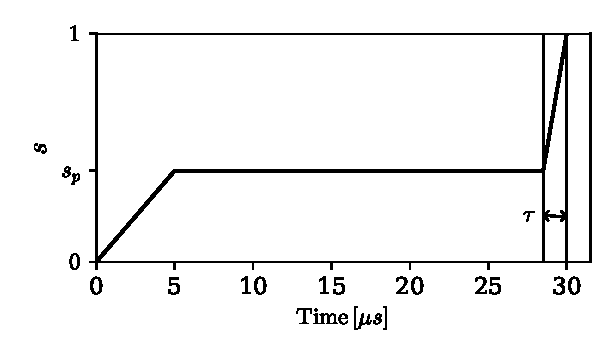
\includegraphics[width=0.55\textwidth]{../plots/pause_schedule.pdf}
    \captionsetup{width=0.9\textwidth}
    \vspace*{-0.4cm}
    \caption{The pause annealing schedule changes the parameter $s$ to a value of $s_p$,
    where the simulation parameters match the physical parameters of the system that we want to simulate. We let the
    system thermalize with the environment and then turn the transverse field off as quickly as the device
    allows. This freezes the state of the system and enables us to measure it.}
    \vspace*{-0.3cm}
    \label{fig:pause_anneal_schedule}
\end{figure}
The main idea is to start with a large transverse field ($s = 0$) and change the parameter $s$ to value $s_p$,
where the simulation parameters match the physical parameters of the system we want to simulate.
The system then evolves at $s_p$ according to the TFIM Hamiltonian and thermalizes with the environment,
which usually takes a few microseconds on a D-Wave processor. After that, we turn the transverse field off as quickly
as the device allows, and we measure the state of the system, thus obtaining a sample. Rapid parameter changes
like this are called quenches. If the quench were instantaneous, it would immitate a projective measurement~\cite*{king2021scaling} and
the output would be a sample from the thermal distribution, associated with the TFIM Hamiltonian at $s_p$ and
temperature $T$ set by the dilution refrigerator. The success of this method depends on two factors:
The ability of the hardware to thermalize to the desired thermal state and the annealing rate during
the quench being fast enough to prevent any changes to the state. We can satisfy the first requirement
by pausing for long enough~\cite*{venuti2016adiabaticity}, but the second requirement can not be satisfied with the current hardware.
In fact, only quenches that are very slow compared to the typical energy scale of the system are currently
possible --- the typical product between the energy of the system $E$ and the time scale of the final
quench $\tau$ is of the order $E \tau / \hbar \sim 10^3$ (recent experiments by the D-Wave team
have been performed with quench times comparable to the typical energy scale of the system~\cite{king2022coherent},
but this feature is not yet commercially available). We therefore expect the state of the system to change
significantly during the final quench and the measured state to not present a sample from the thermal distribution.
Because the transverse magnetic field strength, which is responsible for the quantum fluctuations of spins and
therefore for the reduction of magnetic order in the system, is decreased during this period, the magnetization
in the obtained sample tends to be overestimated. There is no circumventing this problem and
we have to take it into account when analyzing the results of the simulations~\cite*{king2021scaling}.

\hspace*{0.3cm}
An example of magnetization overestimation for the antiferromagnetic ($J_{ij} = J$) TFIM on the cubic lattice is shown in Fig.
\ref{fig:magnetization_overestimation}. The dimensionless transverse field strength was set to $A(s) / B(s) = 2$
and the bias magnetic fields were set to $h_i = 0$ for all $i$. The experiment was carried out on a D-Wave Advantage6.3
processor and was compared to a quantum Monte Carlo simulation, which is a classical sampling algorithm that
is usually used to verify the results of quantum annealers. We discuss this below.
\begin{figure}[!htb]
    \centering
    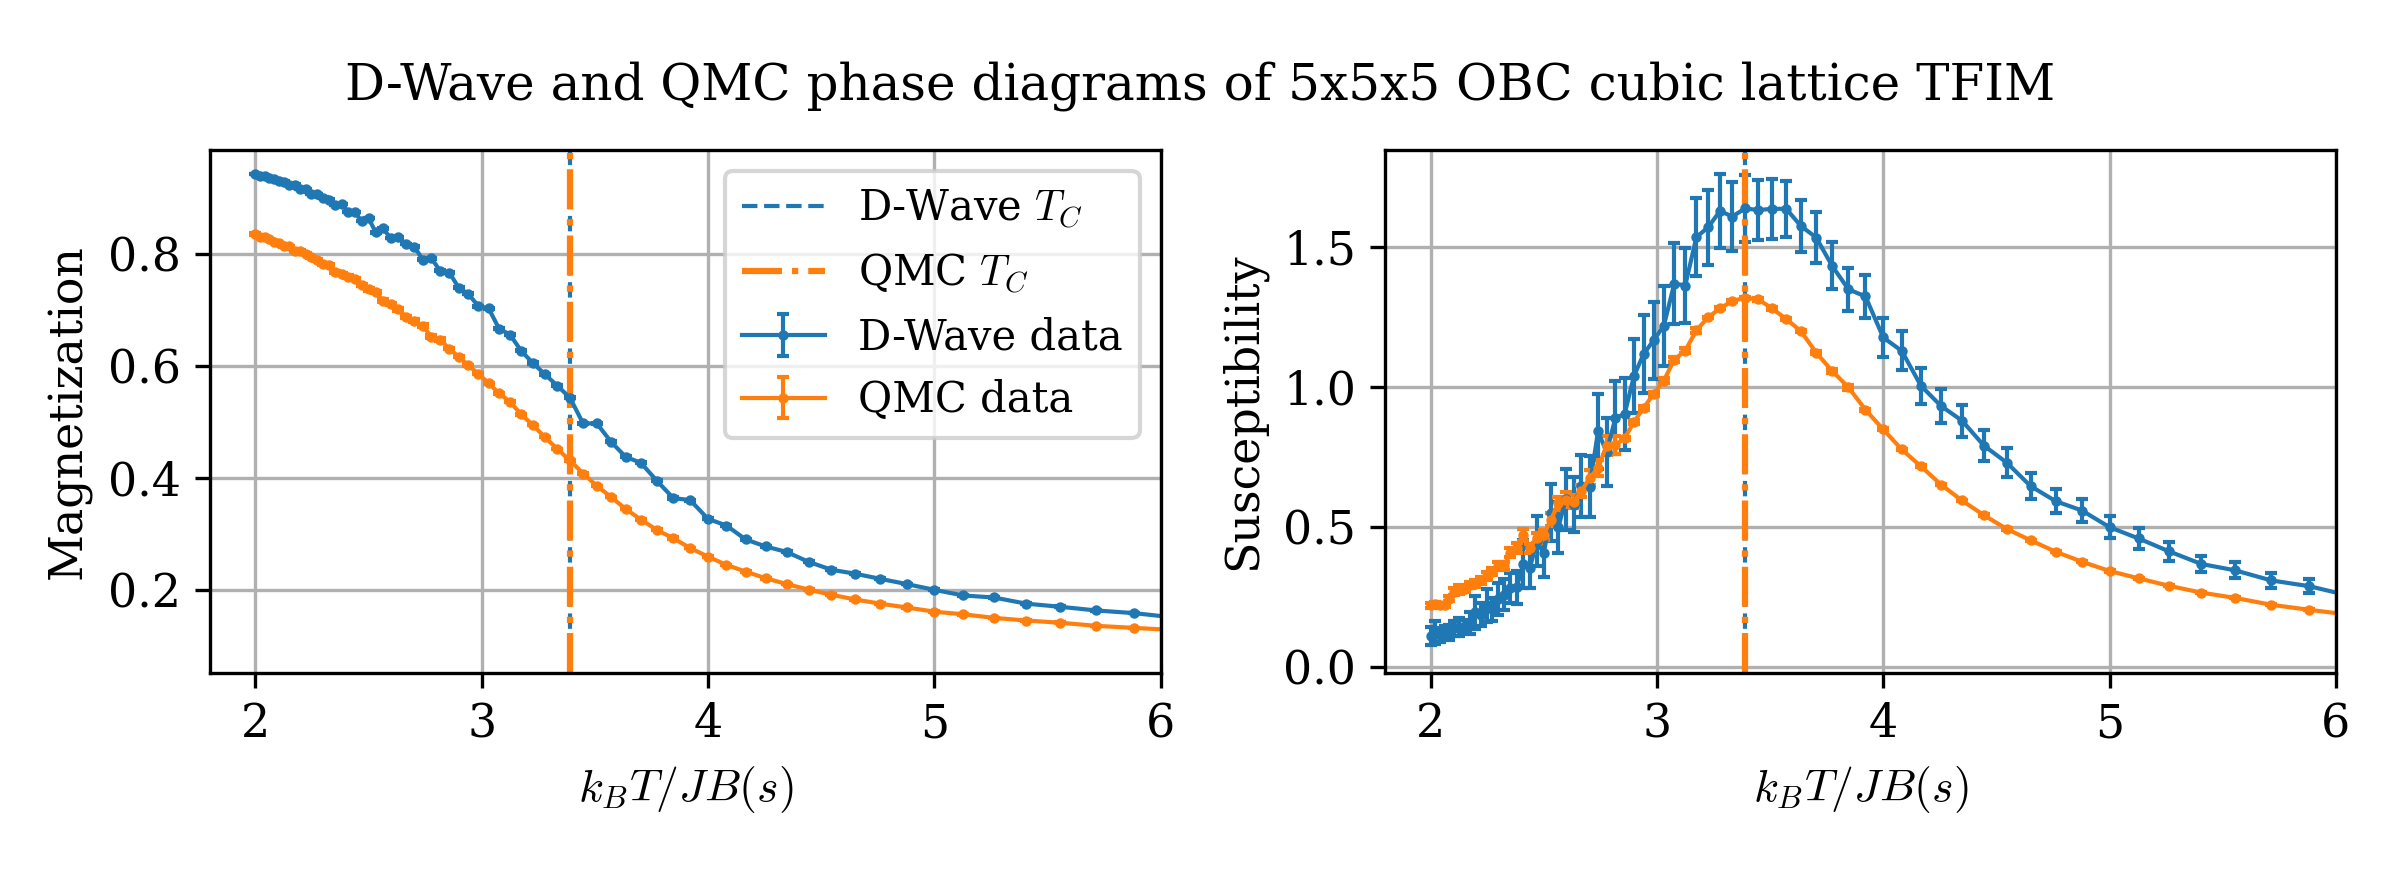
\includegraphics[width=\textwidth]{../plots/dwave_vs_mcmc-5x5x5_gamma2.png}
    \captionsetup{width=0.9\textwidth}
    \caption{(left) Magnetization overestimation for the antiferromagnetic TFIM Hamiltonian on a $5 \times 5 \times 5$
    cubic lattice with transverse field strength $A(s) / B(s) = 2$ in the absence of any bias magnetic fields, $h_i = 0$ for all $i$.
    (right) Magnetic susceptibility allows us to determine the phase transition temperature (vertical lines),
    which is the same for both techniques.}
    \label{fig:magnetization_overestimation}
\end{figure}

\hspace*{0.3cm}
Even though the pause annealing schedule is far from ideal, the results are remarkably accurate in some range of parameters,
especially for determining the phase transition temperatures (Fig. \ref{fig:magnetization_overestimation}).
This encourages us to continue using the quantum annealer for equilibrium simulations of quantum systems.
We expect the results to worsen as the transverse field strength increases due to the longer final quench.

\hspace*{0.3cm}
Now that we have discussed the sampling process on quantum annealers, we can explore whether they
offer any computational advantage over classical computers for simulating the equilibrium properties
of quantum systems. 


\subsection*{Quantum Monte Carlo sampling} \label{sec:qmc}
\hspace*{0.3cm}
When inventing a new computational model, it is important to know what kind of problems it can solve and
how efficiently it can solve them. Classically, the most widely used algorithm for producing thermal
samples is the path integral Monte Carlo (PIMC) method.
The main idea is to rewrite the quantum partition function $Z = \Tr \left( \exp(-\beta H) \right)$ as a partition function
of a classical Ising system in one more dimension using the Trotter-Suzuki decomposition.
States are then sampled according to the classical partition function, using the Metropolis algorithm for example.
Once the states are sampled, the expectation values of observables can be computed.

\hspace*{0.3cm}
When modeling a quantum spin-$1/2$ system on a classical computer, we usually express the operators in the Hamiltonian
as matrices, expressed in the so called computational basis with basis vectors $\ket*{0}$ and $\ket*{1}$ (eigenstates of the
$\sigma^z$ operator). This is usually done when the problem is so complex that we do not know any other basis in
which the Hamiltonian would take a simpler form. For example, the Hamiltonian matrix is particularly simple in the Hamiltonian eigenbasis (diagonal),
but for large problems, we want to avoid diagonalizing the Hamiltonian, so we simply express it in the computational basis.
In this basis, all of the off-diagonal elements in the TFIM Hamiltonian [Eq.~\eqref{eq:QA_ham_full}] are non-positive,
which makes the transition probabilities between computational states in QMC non-negative --- there is no interference
between the computational basis states~\cite*{albash2018adiabatic}. Processes with non-negative
transition probabilities can be modeled on a classical computer using a stochastic algorithm
like the Metropolis algorithm. We call such Hamiltonian stoquastic: 
A stoquastic Hamiltonian is a quantum Hamiltonian, which can be modelled by a stochastic process.

\hspace*{0.3cm}
The stoquasticity of the annealing Hamiltonian [Eq.~\eqref{eq:QA_ham_full}] therefore allows for efficient simulation
of thermal properties of quantum annealers on classical computers~\cite*{bravyi2006complexity}.
By efficient we mean that the computational cost of the simulation scales polynomially with the number of lattice sites.
This is why current generations quantum annealers are believed not to offer
a large computational advantage over classical computers for simulating equilibrium properties of
quantum systems~\cite{crosson2021prospects}. However, there is some evidence that the time it takes for
the TFIM to thermalize, grows slower with the number of lattice sites for QA than PIMC on some problems~\cite*{king2021scaling},
so maybe we will be able to surpass the classical sampling methods with the construction of larger annealers.
Currently, PIMC equilibrium simulations of the largest systems that fit on a D-Wave device are still
routinely performed on classical computers, despite this scaling advantage~\cite*{king2021scaling}. This is one of the reasons for
the shift of focus of research on quantum annealers towards simulating the dynamics of quantum systems~\cite{king2024computational, king2023quantum, king2022coherent}.

\hspace*{0.3cm}
One way to increase the computational power of quantum annealers is to use non-stoquastic Hamiltonians,
which are not efficiently simulable by QMC methods. This can be achieved by adding a $\sigma^x \sigma^x$ or
$\sigma^y \sigma^y$ coupling to the TFIM Hamiltonian \eqref{eq:QA_ham_full}. The implementation of such
coupling was already demonstrated~\cite*{ozfidan2020demonstration}, but the D-Wave has not decided to
commercialize it yet.

\section{Conclusion} \label{sec:conclusion}
\hspace*{0.3cm}
Even though quantum annealing is technically a universal model of quantum computation, we believe that its usage will
remain limited to solving optimization problems and simulating quantum systems. The main reason for this is that
quantum annealers are only able to represent a certain class of parametrized Hamiltonians and it is not always
easy to map a problem of interest onto this class. In other words, gate model quantum computers are simply
a more natural choice for simulating a general quantum evolution. That being said, many problems of interest
can be cast as optimization problems and quantum annealers have been successfully used to solve them.
But even more important, in our view, is the ability to use quantum annealers for simulation of quantum systems
today and challenge the limits of classical computers in this domain. Equilibrium simulations might still
be easier on classical computers, but the real interest currently lies in simulating the closed-system
dynamics of quantum systems, since there is no known efficient classical algorithm for this task.
While we await scalable gate model quantum computers, quantum annealing provides an exciting opportunity
to explore the properties of quantum systems that are not easily accessible using classical computers.


\printbibliography

% \begin{figure}[!htb]
    % \centering
%     \begin{subfigure}
%         \includegraphics[width=0.45\textwidth]{}
%     \end{subfigure}
%     \begin{subfigure}
%         \includegraphics[width=0.45\textwidth]{}
%     \end{subfigure}
%     \captionsetup{width=0.9\textwidth}
%     \caption{}
%     \label{fig:}
% \end{figure}

% \begin{figure}[!htb]
%     \centering
%     \includegraphics[width=0.8\textwidth]{}
%     \captionsetup{width=0.9\textwidth}
%     \caption{}
%     \label{fig:}
% \end{figure}

\end{document}
